\section{Career Path Results}
\label{sect:career-path-results}
Examples of the objects returned by the career path graph portion of the
ProGENitor code are shown below.  Each example does not contain a complete set
of data as that would be too much to show in this report.

\subsection{Node Edge Results}
In the node edge object, an array of node edges is returned.  Each element
of the array contains a starting node and an ending node for the transition. 
Additionally, the array element also contains a transition frequency.  The
transition frequency indicates how often the transition occurs.  To
prevent exposure of user data, these transitions are scaled to a value
ranging from 0 and 10.

\begin{tt}
\begin{footnotesize}
\noindent\{"Node Connections":\\*
\{"node A":"Bachelors","node B":"Masters","transition frequency":6\},\\*
\{"node A":"Masters","node 	B":"Circuit Designer","transition frequency":7\},\\*
\{"node A":"Circuit Designer","node B":"Block 	Owner","transition
 frequency":8\},\\* 
\{"node A":"Block Owner","node B":"Design Owner","transition frequency":9\},\\*
\ldots\\* 
\{"node A":"Coder","node B":"Function Lead","transition frequency":0\},\\*
\{"node A":"Function Lead","node B":"Masters","transition frequency":0\}\},\\*
\end{footnotesize}
\end{tt}


\subsection{Node Ordering JSON Results}
In the node ordering object, an array containing the order which the nodes
should be display is returned.  Each element of the array contains a node name
and the order number it should be displayed.  Thus, the nodes with an order of
1 should be the first nodes displayed in the career path graph, then
moving sequentially up, each node in the group should be displayed until the
final node group is displayed.  This will allow the graph to flow with minimum
edges flowing in the reverse direction.

\begin{tt}
\begin{footnotesize}
\noindent \{"Node Ordering":\\*
	\indent\{"node	name":"Timing","order":"2"\},\\*
	\indent\{"node name":"Signal Integrity","order":"2"\},\\*
	\indent\{"node name":"Platform Chief Engineer","order":"7"\},\\*
	\indent\{"node name":"PhD","order":"5"\},\\*
	\indent\{"node name":"Entry Coder","order":"1"\},\\*
	\indent\ldots\\*
	\indent\{"node name":"Block Owner","order":"6"\},\\*
	\indent\{"node name":"Chiplet Designer","order":"1"\}]\},\\*
\end{footnotesize}
\end{tt}

\subsection{Node Details Results}
In the node detail object, an array containing all of the various nodes
will be returned.  Each node will be a nested object containing an array of data
points.  Examples of these data points are titles, companies, time spent at the
node, and any other points of interest within the database.  Each of these data
points will be an object that also contains a nested array.  This array
will then contain data about each data point, broken down into the percentage of
users who matched a specific piece of information for that data point.  For
example, shown below is a data point for the companies that users worked for
when they worked at a Timing job.  To protect user data, this is not shown as
number of users, but as the percentage of users who spent time working for one
company versus all users who spent time working at that particular job.  To
avoid returning millions of entries, a threshold is set such that only
statistically relevant data is returned and everything else is lumped into an
``other'' group.  This ``other'' group would then contain the total user data
that did not meet the threshold.  Finally, an object containing any significant data
points is also returned.

ProGENitor compares the users who reached the goal against all users who passed
through the node to determine what was statistically different from the users
who reached the target goal.  These differences are listed in the significant
data object. In the example below, the significant data point is that 100\% of
the users who passed through this node and reached the goal node worked for
Verizon.  This is significant because only 11\% of the the users who spent time
in this node worked for Verizon.  Thus, working for Verizon in the Timing job is
an important step to reaching the goal node.  Significance is flagged whenever
the users who reached the goal, had a data point occur 5\% more than then
everyone who passed through the node.  This value could easily be modified by
the company deploying ProGENitor if a greater difference was required for significance.

\pagebreak
\begin{tt}
\begin{footnotesize}
\noindent \{"Nodes Data":\\*
	\indent \{"Node Name":"Timing","Node Data":\\*
		\indent \{"Data Breakout":\\*
		\indent \indent	\{"name":"Other","value":"0.9174312\%"\}\\*
		\indent	\indent \{"name":"Timing\_all","value":"100.0\%"\},\\*
		\indent	"Data Point Name":"title"\},\\*
		\indent\{"Data Breakout":\\*
		\indent	\indent	\{"name":"Verizon","value":"100.0\%"\},\\*
		\indent	\indent	\{"name":"Verizon\_all","value":"11.33721\%"\},\\*
		\indent	\indent	\{"name":"Cisco Systems\_all","value":"12.790698\%"\},\\*
		\indent	\indent	\{"name":"Boeing\_all","value":"7.5581393\%"\},\\*
		\indent	\indent	\{"name":"Hewlit-Packard\_all","value":"8.139535\%"\},\\*
		\indent	\indent	\{"name":"IBM\_all","value":"7.2674417\%"\},\\*
		\indent	\indent	\{"name":"General Motors\_all","value":"8.72093\%"\},\\*
		\indent	\indent	\{"name":"General Electric\_all","value":"7.2674417\%"\},\\*
		\indent	\indent	\{"name":"Microsoft\_all","value":"8.72093\%"\},\\*
		\indent	\indent	\{"name":"Intel\_all","value":"8.72093\%"\},\\*
		\indent	\indent	\{"name":"Lockheed Martin\_all","value":"11.046512\%"\},\\*
		\indent	\indent	\{"name":"AT\&T\_all","value":"8.430233\%"\},\\*
		\indent"Data Point Name":"company"\},\\*
		\indent\ldots\\*
		\indent \{"Significant":Verizon\}\},\\*
\end{footnotesize}
\end{tt}

\subsection{Example Career Path 1}
With the ProGENitor tool, several examples of functionality can easily be
demonstrated.  In the first example, consider a user that is interested in
what it takes to become a partner in an architecture firm.  The user would submit the query on
partner and the career graph shown in Figure \ref{fig:partner nodal map} would
be returned.

\usetikzlibrary{shapes,arrows,chains}

\begin{figure}[H]
	\centering
  
% Start the picture
\resizebox {108mm} {!} {
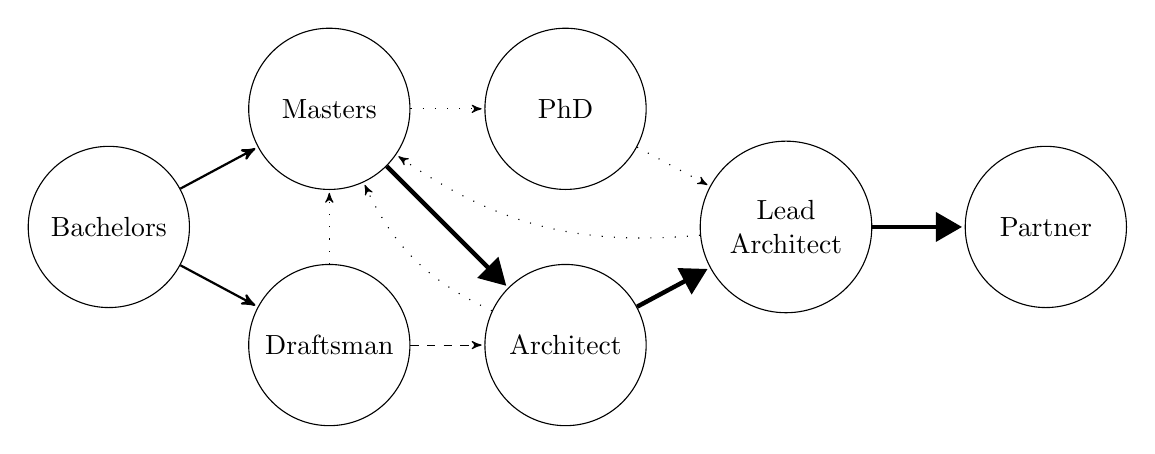
\begin{tikzpicture}[%
    >=triangle 60,              % Nice arrows; your taste may be different
    start chain=going below,    % General flow is top-to-bottom
    node distance=3mm and 28mm, % Global setup of box spacing
    every join/.style={norm},   % Default linetype for connecting boxes
    ]
% ------------------------------------------------- 
% A few box styles 
% <on chain> *and* <on grid> reduce the need for manual relative
% positioning of nodes
\tikzset{
  base/.style={draw, on chain, on grid, align=center, minimum height=2ex},
  node/.style={base, circle, text width=5em},
  % Connector line styles for different parts of the diagram
  norm/.style={->, draw},
  tn/.style={->,>=stealth',shorten >=1pt, loosely dotted},
  nm/.style={->,>=stealth',shorten >=1pt,dashed},
  to/.style={->,>=stealth',shorten >=1pt,thick},
  tk/.style={->,shorten >=1pt,ultra thick},
  it/.style={font={\small\itshape}}
}
% -------------------------------------------------
% Start by placing the nodes
\node [node] (a) {Bachelors};
% Use join to connect a node to the previous one 
\node [node, right = of a, yshift=15mm] (b) {Masters};
\node [node, right = of a, yshift=-15mm] (c) {Draftsman}; 
\node [node, right = of b, xshift=2mm](d) {PhD};
\node [node, right = of c, xshift=2mm](e) {Architect};
\node [node, right = of e, yshift=15mm](f) {Lead Architect};
\node [node, right = of f, xshift=5mm](g) {Partner};

\draw[to] (a) to (c);%Bachelors,Draftsman,4
\draw[tn] (c) to (b);	%Draftsman,Masters,1
\draw[tk] (b) to (e);	%Masters,Architect,7
\draw[tk] (e) to (f);	%Architect,Lead Architect,7
\draw[tk] (f) to (g);	%Lead Architect,Partner,7
\draw[to] (a) to (b);	%Bachelors,Masters,5
\draw[tn] (b) to (d); %Masters,PhD,0
\draw[tn] (d) to (f);	%PhD,Lead Architect,0
\draw[nm] (c) to (e);	%Draftsman,Architect,2
\draw[tn] (e) to [bend left=20] (b);	%Architect,Masters,0
\draw[tn] (f) to [bend left=20] (b);	%Lead
% Architect,Masters,0

% -------------------------------------------------
\end{tikzpicture}
}

	\caption{Career Path Graph}
	\label{fig:partner nodal map}
\end{figure}

This graph quickly shows the user that a bachelor's degree is required.  Next
the users can see that a master's degree could help them move into an architect
role right away versus starting out as a draftsman.  In either case, both
options can eventually lead to the desired partner position, with no major
indicator which one yielded a higher likelihood of achieving the goal.  It also
shows that it is rare for someone to return for a master's degree once they've
entered the workforce and doing so later in your career can actually set the
users back, if they've moved up past the architect position.  Finally, very
few people who reached the partner status also obtained a PhD, showing that this
is not a common path to reaching partner, but still is an option that could be
pursued.

Next, the user could select one of the nodes to pull up additional information
about that node.  The three pie charts below in Figure \ref{fig:Lead Arch} show
the information that would be returned if the user were to select the lead
architect node.  These charts show that there were five key employers for all of
the users who reached partner.  They also show that most of the partners were
lead architects for less than five years, and it became increasingly rare to
reach partner after this time.  The data also shows that no particular city had
lead architects getting promoted to partner more frequently.  Thus, any lead
architects looking at this data would know to reach partner they need to be
focused on doing so within the five year window or they can expect their chances
of doing so to diminish over time.  Also, they should know that where and who
they work for is not important, as long as they work for one of the five
companies shown.

Alternatively, the user could click on the master's degree node, to see more
information about these users.  In doing so, the data generated immediately
shows everyone who got a Master's degree did so in a single year with a
specialization in Infrastructure and the only variation being in the school
attended.  In this case there were eight different schools attended, but none
were attended at a more significant frequency than the rest.  Thus, the user
could immediately know if they wished to reach partner and do so by obtaining their
master's degree, they need to get an Infrastructure degree within a year by
attending one of these eight schools.


\begin{figure}[H]
\centering

\hspace*{-3cm}\begin{subfigure}[h]{.5\textwidth}
	\centering
	% Pie chart with colors
	% Author: Henri Menke
	\def\angle{0}
	\def\radius{3}
	\def\cyclelist{{"orange","blue","red","green"}}
	\newcount\cyclecount \cyclecount=-1
	\newcount\ind \ind=-1
	\resizebox {88mm} {!} {
	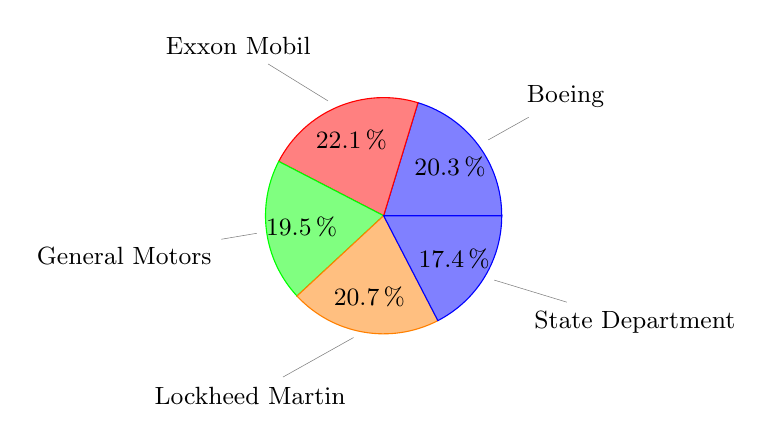
\begin{tikzpicture}[nodes = {font=\small},scale=.5]
  		\foreach \percent/\name in {
      		20.3/Boeing,
      		22.1/Exxon Mobil,
      		19.5/General Motors,
      		20.7/Lockheed Martin,
      		17.4/State Department
    	} {
      		\ifx\percent\empty\else               % If \percent is empty, do nothing
        	\global\advance\cyclecount by 1     % Advance cyclecount
        	\global\advance\ind by 1            % Advance list index
        	\ifnum3<\cyclecount                 % If cyclecount is larger than list
          	\global\cyclecount=0              %   reset cyclecount and
          	\global\ind=0                     %   reset list index
        	\fi
        	\pgfmathparse{\cyclelist[\the\ind]} % Get color from cycle list
        	\edef\color{\pgfmathresult}         %   and store as \color
        	% Draw angle and set labels
        	\draw[fill={\color!50},draw={\color}] (0,0) -- (\angle:\radius)
          		arc (\angle:\angle+\percent*3.6:\radius) -- cycle;
        	\node at (\angle+0.5*\percent*3.6:0.7*\radius) {\percent\,\%};
        	\node[pin=\angle+0.5*\percent*3.6:\name]
          		at (\angle+0.5*\percent*3.6:\radius) {};
        	\pgfmathparse{\angle+\percent*3.6}  % Advance angle
        	\xdef\angle{\pgfmathresult}         %   and store in \angle
      		\fi
    	};
	\end{tikzpicture}
	}

	\caption{Company}
	\label{fig:node pie comp}
\end{subfigure}

\begin{subfigure}{.5\linewidth}
	\centering
	% Pie chart with colors
	% Author: Henri Menke
	\def\angle{0}
	\def\radius{3}
	\def\cyclelist{{"orange","blue","red","green"}}
	\newcount\cyclecount \cyclecount=-1
	\newcount\ind \ind=-1
	\resizebox {68mm} {!} {
	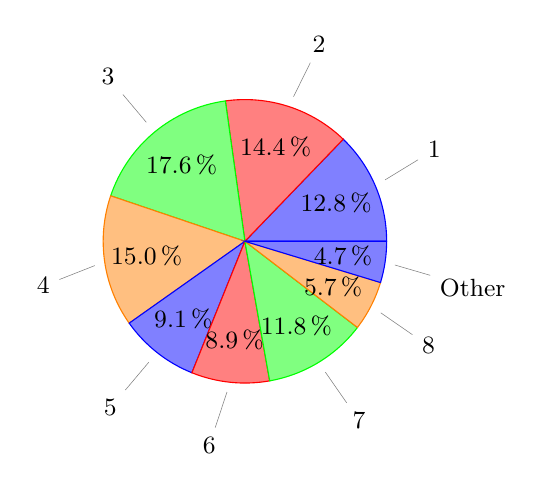
\begin{tikzpicture}[nodes = {font=\small},scale=.6]
  		\foreach \percent/\name in {
      		12.8/1,
      		14.4/2,
      		17.6/3,
      		15.0/4,
      		9.1/5,
      		8.9/6,
      		11.8/7,
      		5.7/8,
      		4.7/Other       
    	} {
      	\ifx\percent\empty\else               % If \percent is empty, do nothing
        \global\advance\cyclecount by 1     % Advance cyclecount
        \global\advance\ind by 1            % Advance list index
        \ifnum3<\cyclecount                 % If cyclecount is larger than list
        \global\cyclecount=0              %   reset cyclecount and
        \global\ind=0                     %   reset list index
        \fi
        \pgfmathparse{\cyclelist[\the\ind]} % Get color from cycle list
        \edef\color{\pgfmathresult}         %   and store as \color
        % Draw angle and set labels
        \draw[fill={\color!50},draw={\color}] (0,0) -- (\angle:\radius)
          	arc (\angle:\angle+\percent*3.6:\radius) -- cycle;
        \node at (\angle+0.5*\percent*3.6:0.7*\radius) {\percent\,\%};
        \node[pin=\angle+0.5*\percent*3.6:\name]
          	at (\angle+0.5*\percent*3.6:\radius) {};
        \pgfmathparse{\angle+\percent*3.6}  % Advance angle
        \xdef\angle{\pgfmathresult}         %   and store in \angle
      	\fi
    };
	\end{tikzpicture}
	}

	\caption{Years Spent at Job}
	\label{fig:node pie job}
\end{subfigure}

\hspace*{-7cm}\begin{subfigure}[h]{.25\linewidth}

	% Pie chart with colors
	% Author: Henri Menke
	\def\angle{0}
	\def\radius{3}
	\def\cyclelist{{"orange","blue","red","green"}}
	\newcount\cyclecount \cyclecount=-1
	\newcount\ind \ind=-1
	\resizebox {98mm} {!} {
	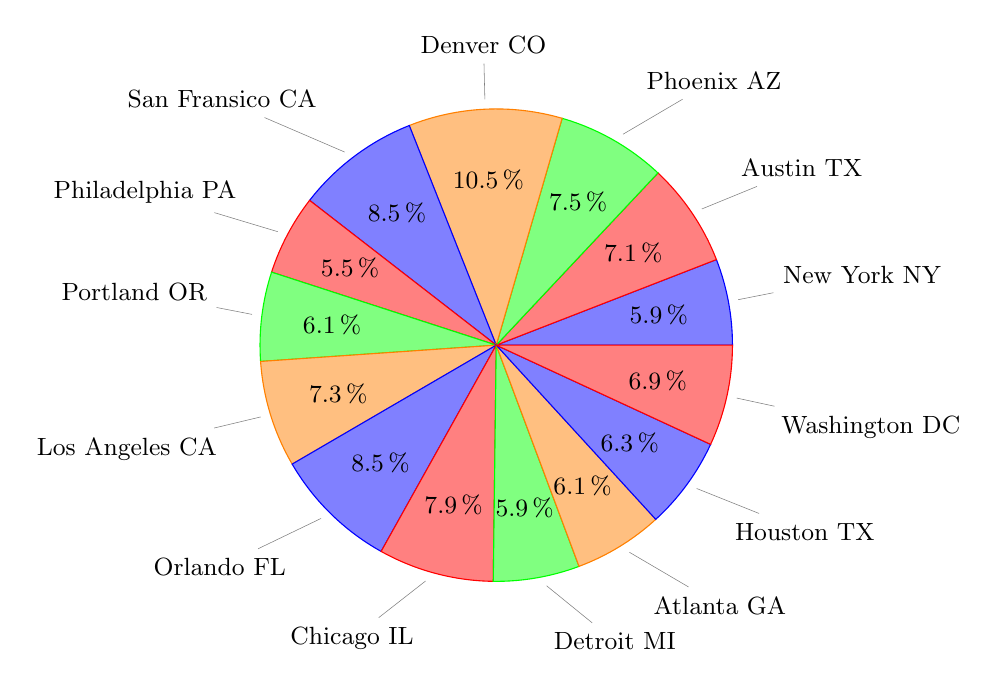
\begin{tikzpicture}[nodes = {font=\small}]
  		\foreach \percent/\name in {
			5.9/New York NY,
			7.1/Austin TX,
			7.5/Phoenix AZ,
			10.5/Denver CO,
			8.5/San Fransico CA,
			5.5/Philadelphia PA,
			6.1/Portland OR,
			7.3/Los Angeles CA,
			8.5/Orlando FL,
			7.9/Chicago IL,
			5.9/Detroit MI,
			6.1/Atlanta GA,
			6.3/Houston TX,
			6.9/Washington DC      
    	} {
      	\ifx\percent\empty\else               % If \percent is empty, do nothing
        \global\advance\cyclecount by 1     % Advance cyclecount
        \global\advance\ind by 1            % Advance list index
        \ifnum3<\cyclecount                 % If cyclecount is larger than list
        \global\cyclecount=0              %   reset cyclecount and
        \global\ind=0                     %   reset list index
        \fi
        \pgfmathparse{\cyclelist[\the\ind]} % Get color from cycle list
        \edef\color{\pgfmathresult}         %   and store as \color
        % Draw angle and set labels
        \draw[fill={\color!50},draw={\color}] (0,0) -- (\angle:\radius)
          	arc (\angle:\angle+\percent*3.6:\radius) -- cycle;
        \node at (\angle+0.5*\percent*3.6:0.7*\radius) {\percent\,\%};
        \node[pin=\angle+0.5*\percent*3.6:\name]
          	at (\angle+0.5*\percent*3.6:\radius) {};
        \pgfmathparse{\angle+\percent*3.6}  % Advance angle
        \xdef\angle{\pgfmathresult}         %   and store in \angle
      	\fi
    	};
	\end{tikzpicture}
	}
	
	\caption{Job Location}
	\label{fig:node pie job}
\end{subfigure}

\caption{Lead Architect}
\label{fig:Lead Arch}
\end{figure}

The proper functionality of the algorithms can be demonstrated trough
several modifications to the data fed into the synthetic data generation script.
With the following modifications, it will be shown that the results
ProGENitor produce align with the expected changes. First, a second
specialization is added to Civil Engineering but it is occurs a third of the
time.  This is done by adding the following line to the Masters text file.

	\indent
	\begin{footnotesize}\begin{tt}{Civil:Infrastructure,Energy,Infrastructure}\\*\end{tt}\end{footnotesize}

\noindent Next, an additional node, junior partner is added prior to partner. 
This is done by modify the titles text file.  To make this change, the simple
replacement of one line with two new lines was needed.
	
	\begin{footnotesize}
	\indent Remove: \begin{tt}Lead Architect:Partner\\*\end{tt}
	\indent Add: \begin{tt}Lead Architect:Junior Partner\\*\end{tt}
	\indent Add: \begin{tt}Junior Partner:Partner\\*\end{tt}
	\end{footnotesize}
	
\noindent Finally, the likelihood of someone obtaining a master's degree was
reduced by incrementing a probability variable by 2 in the data generation
script.



\usetikzlibrary{shapes,arrows,chains}

\begin{figure}[H]
	\centering
  
% Start the picture
\resizebox {140mm} {!} {
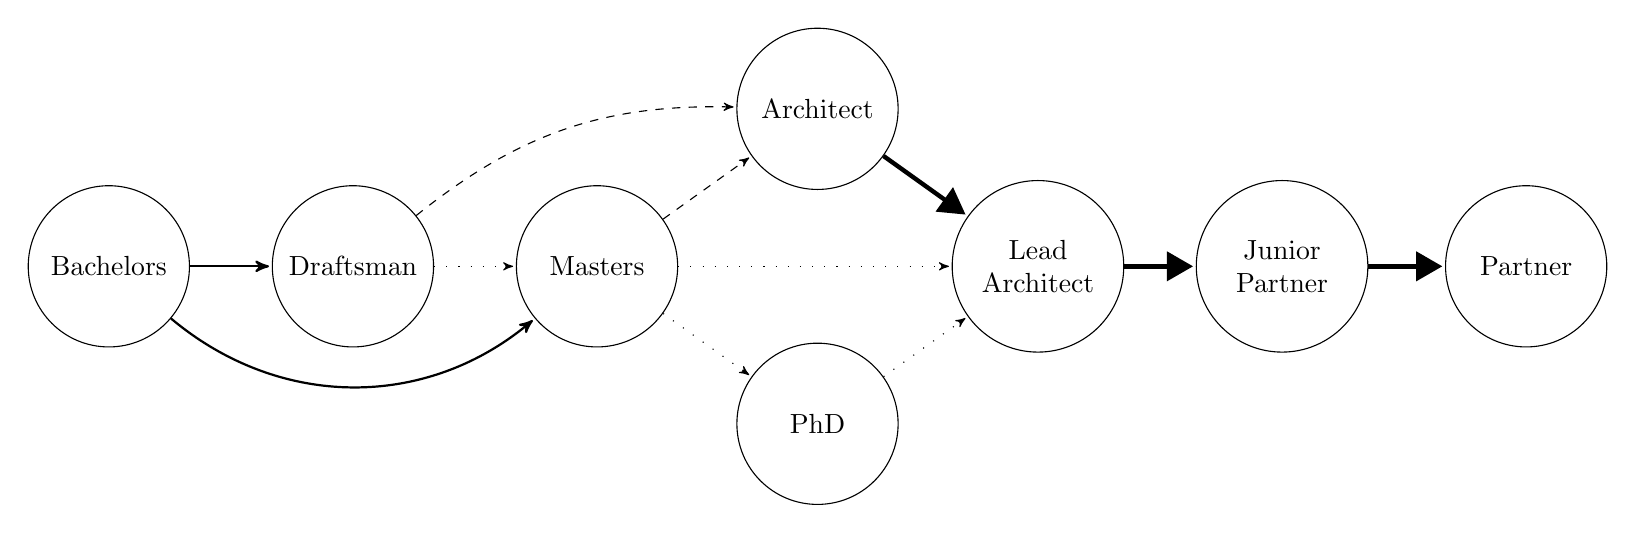
\begin{tikzpicture}[%
    >=triangle 60,              % Nice arrows; your taste may be different
    start chain=going below,    % General flow is top-to-bottom
    node distance=4mm and 28mm, % Global setup of box spacing
    every join/.style={norm},   % Default linetype for connecting boxes
    ]
% ------------------------------------------------- 
% A few box styles 
% <on chain> *and* <on grid> reduce the need for manual relative
% positioning of nodes

\tikzset{
  base/.style={draw, on chain, on grid, align=center, minimum height=2ex},
  node/.style={base, circle, text width=5em},
  % Connector line styles for different parts of the diagram
  norm/.style={->, draw},
  tn/.style={->,>=stealth',shorten >=1pt, loosely dotted},
  nm/.style={->,>=stealth',shorten >=1pt,dashed},
  to/.style={->,>=stealth',shorten >=1pt,thick},
  tk/.style={->,shorten >=1pt,ultra thick},
  it/.style={font={\small\itshape}}
}
% -------------------------------------------------
% Start by placing the nodes
\node [node, xshift=-10mm] (a) {Bachelors};
% Use join to connect a node to the previous one 
\node [node, right = of a, xshift=3mm] (b) {Draftsman};
\node [node, right = of b, xshift=3mm] (c) {Masters}; 
\node [node, right = of c, yshift=20mm] (d) {Architect};
\node [node, right = of c, yshift=-20mm] (e) {PhD};
\node [node, right = of e, yshift=20mm] (f) {Lead Architect};
\node [node, right = of f, xshift=3mm] (g) {Junior Partner};
\node [node, right = of g, xshift=3mm] (h) {Partner};

\draw[to] (a) to (b);		%Bachelors,Draftsman,5
\draw[nm] (b) to [bend left=20] (d);		%Draftsman,Architect,4
\draw[tk] (d) to (f);		%Architect,Lead Architect,7
\draw[tk] (f) to (g);	%Lead Architect,Junior Partner,10
\draw[tk] (g) to (h);	%Junior Partner,Partner,10
\draw[to] (a) to [bend right=40] (c);		%Bachelors,Masters,4
\draw[nm] (c) to (d); 	%Masters,Architect,2
\draw[tn] (c) to (f);		%Masters,Lead Architect,1
\draw[tn] (c) to (e);		%Masters,PhD,0
\draw[tn] (e) to (f);		%PhD,Lead Architect,0
\draw[tn] (b) to (c);		%Draftsman,Masters,0

% -------------------------------------------------
\end{tikzpicture}
}

	\caption{Modified Career Path Graph}
	\label{fig:mod partner nodal map}
\end{figure}

With these changes in place, the new career path graph for achieving the partner
position shows the expected changes.  The new node step of junior partner is
present and it also shows the reduction of users obtain a master's degree.  In
the case of users transitioning from a bachelor's to master's degree, it is not
clear from the edges, but by looking at the data in the returned object, the
frequency did decrease by 10\%.  In the detailed data for the master's degree
node, the Infrastructure degree makes up approximately 2/3rds of the total
degrees.  This is shown in the object return for the masters node with the
following text:

\begin{tt}
\begin{footnotesize}
\indent Data Breakout"\\*
\indent \indent \indent \{"name":"Infrastructure","value":"61.50794\%"\},\\*
\indent \indent \indent \{"name":"Energy","value":"38.49206\%"\}
\end{footnotesize}
\end{tt}

\noindent Additionally, both Infrastructure and Energy would be returned as
significant pieces of data, as they occurred much less frequently for the users
who traveled through this master's degree node and did not reach the partner
node.

\subsection{Example Career Path 2 }
In the second example, consider another user who is interested in reaching the
system chief engineering role.  They would input this query into the tool and
Figure \ref{fig:node map sce} would be generated.  From this graph, the user
would quickly be able to see that obtaining an advanced degree was unnecessary
to become a system chief engineer.  They could then delve deeper into each node
if they wanted to learn more about users who did the various jobs that also
became system chief engineers.


\usetikzlibrary{shapes,arrows,chains}

\begin{figure}[H]
	\centering
  
% Start the picture
\resizebox {140mm} {!} {
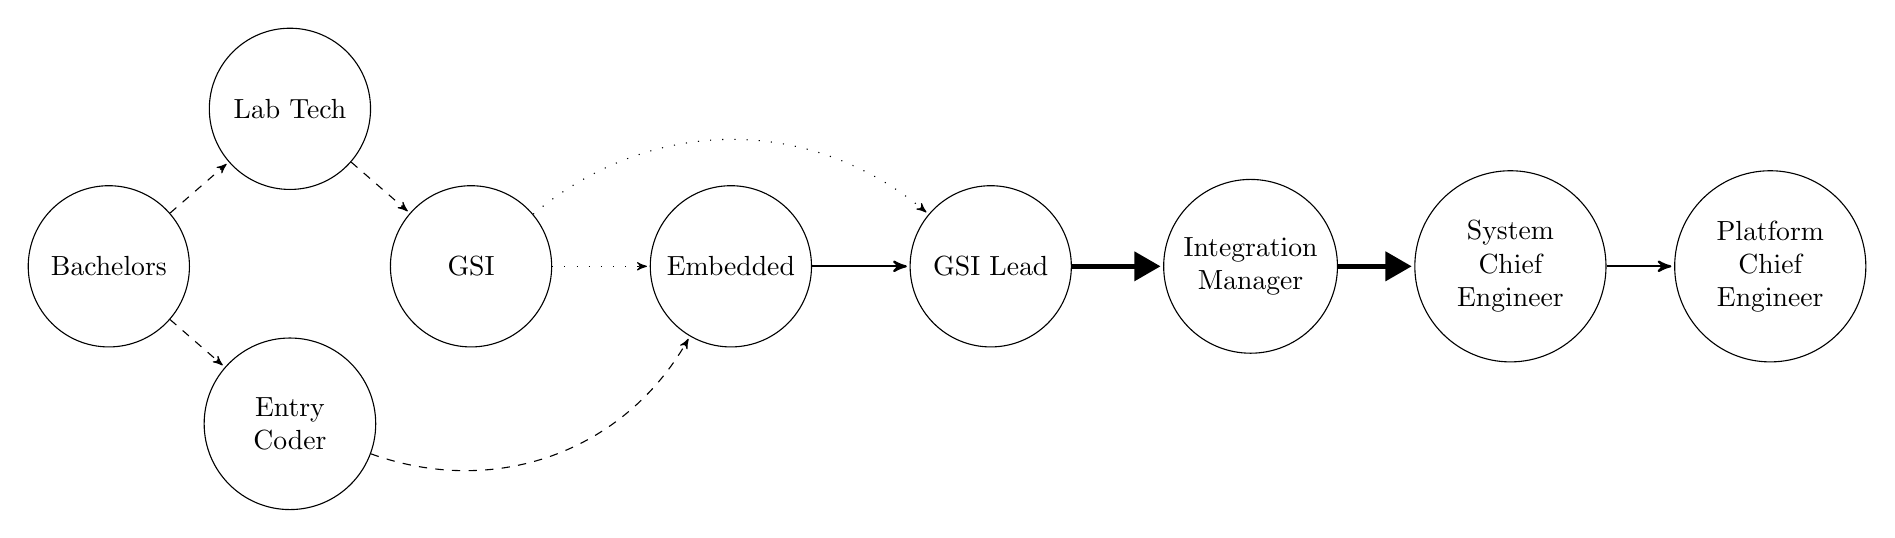
\begin{tikzpicture}[%
    >=triangle 60,              % Nice arrows; your taste may be different
    start chain=going below,    % General flow is top-to-bottom
    node distance=3mm and 28mm, % Global setup of box spacing
    every join/.style={norm},   % Default linetype for connecting boxes
    ]
% ------------------------------------------------- 
% A few box styles 
% <on chain> *and* <on grid> reduce the need for manual relative
% positioning of nodes
\tikzset{
  base/.style={draw, on chain, on grid, align=center, minimum height=2ex},
  node/.style={base, circle, text width=5em},
  % Connector line styles for different parts of the diagram
  norm/.style={->, draw},
  tn/.style={->,>=stealth',shorten >=1pt, loosely dotted},
  nm/.style={->,>=stealth',shorten >=1pt,dashed},
  to/.style={->,>=stealth',shorten >=1pt,thick},
  tk/.style={->,shorten >=1pt,ultra thick},
  it/.style={font={\small\itshape}}
}
% -------------------------------------------------
% Start by placing the nodes

\node [node] (a) {Bachelors};
% Use join to connect a node to the previous one 
\node [node, right = of a,xshift=-5mm,yshift=-20mm] (b) {Entry Coder};
\node [node, right = of a,xshift=-5mm,yshift=20mm] (c) {Lab Tech}; 
\node [node, right = of b,xshift=-5mm,yshift=20mm] (d) {GSI};
\node [node, right = of d,xshift=5mm] (e) {Embedded};
\node [node, right = of e,xshift=5mm] (f) {GSI Lead};
\node [node, right = of f,xshift=5mm] (g) {Integration Manager};
\node [node, right = of g,xshift=5mm] (h) {System Chief Engineer};
\node [node, right = of h,xshift=5mm] (i) {Platform Chief Engineer}; 

\draw[nm] (a) to (c);		%Bachelors,Lab Tech,7
\draw[nm] (c) to (d);		%Lab Tech,GSI,7
\draw[tn] (d) to [bend left=40] (f);		%GSI,GSI Lead,4
\draw[tk] (f) to (g);		%GSI Lead,Integration Manager,14
\draw[tk] (g) to (h);		%Integration Manager,System Chief Engineer,14
\draw[to] (h) to (i);		%System Chief Engineer,Platform Chief Engineer,11
\draw[nm] (a) to (b);		%Bachelors,Entry Coder,7
\draw[nm] (b) to [bend right=40] (e);		%Entry Coder,Embedded,7
\draw[to] (e) to (f);		%Embedded,GSI Lead,10
\draw[tn] (d) to (e);		%GSI,Embedded,3

% -------------------------------------------------
\end{tikzpicture}
}

	\caption{System Chief Engineer Graph}
	\label{fig:node map sce}
\end{figure}

One thing that might also spark an interest in the user is the fact that any
jobs beyond the queried job that the matched users also completed would be shown
as well.  In this case there was one of these such nodes, the platform chief
engineer.  From the node edges it is clear that not all system chief
engineers reached this job.  If the user were interested then instead in the
platform chief engineering role, they could re-run the query.  They would then
be presented with the career graph shown in Figure \ref{fig:node map pce}.  This
is obviously a much more complex graph, but it still yields the same capability
of quickly showing users complex career paths to a particular goal.  In this
case it shows that there are essentially three paths to this job.  The first
path was detailed in the initial query, the second path is through a design
career path, and the third path is through an advanced degree.  What is most
notable about these paths is if the advanced degree path is taken, the initial
jobs the users take don't have much impact, as long as it is within the career realm.
The other notable thing is the most common path taken to getting to the platform
chief engineering job is through the design path.


\usetikzlibrary{shapes,arrows,chains}

\begin{figure}[H]
	\centering
  
% Start the picture
\resizebox {!} {190mm} {
\begin{tikzpicture}[%
    >=triangle 60,              % Nice arrows; your taste may be different
    start chain=going below,    % General flow is top-to-bottom
    node distance=3mm and 28mm, % Global setup of box spacing
    every join/.style={norm},   % Default linetype for connecting boxes
    ]
% ------------------------------------------------- 
% A few box styles 
% <on chain> *and* <on grid> reduce the need for manual relative
% positioning of nodes
\tikzset{
  base/.style={draw, on chain, on grid, align=center, minimum height=2ex},
  node/.style={base, circle, text width=5em},
  % Connector line styles for different parts of the diagram
  norm/.style={->, draw},
  tn/.style={->,>=stealth',shorten >=1pt, loosely dotted},
  nm/.style={->,>=stealth',shorten >=1pt,dashed},
  to/.style={->,>=stealth',shorten >=1pt,thick},
  tk/.style={->,shorten >=1pt,ultra thick},
  it/.style={font={\small\itshape}}
}
% -------------------------------------------------
% Start by placing the nodes

\node [node] (a) {Bachelors};
% Use join to connect a node to the previous one 
\node [node, below = of a,yshift=-30mm,xshift=20mm] (b) {Entry Coder};
\node [node, below = of a,yshift=-30mm,xshift=60mm] (c) {Lab Tech}; 
\node [node, below = of a,yshift=-30mm,xshift=-60mm] (d) {Schematic Entry};
\node [node, below = of a,yshift=-30mm,xshift=-20mm] (e) {Chiplet Designer};
\node [node, below = of d,yshift=-30mm,xshift=40mm] (f) {Timing};
\node [node, below = of d,yshift=-30mm,xshift=120mm] (g) {Signal Integrity};
\node [node, below = of d,yshift=-30mm,xshift=-40mm] (h) {Circuit Designer};
\node [node, below = of d,yshift=-30mm,xshift=80mm] (i) {Coder};
\node [node, below = of d,yshift=-30mm,xshift=0mm] (j) {Schematic Lead};
\node [node, below = of d,yshift=-30mm,xshift=160mm] (k) {GSI};
\node [node, below = of i,yshift=-30mm] (l) {Function Lead};
\node [node, below = of i,yshift=-30mm,xshift=40mm] (m) {Embedded};
\node [node, below = of l,yshift=-30mm,xshift=-40mm] (n) {Masters};
\node [node, below = of l,yshift=-30mm,xshift=40mm] (o) {GSI Lead};
\node [node, below = of n,yshift=-30mm] (p) {PhD};
\node [node, below = of o,yshift=-30mm] (q) {Integration Manager};
\node [node, below = of q,yshift=-30mm] (r) {System Chief Engineer};
\node [node, below = of p,yshift=-30mm] (s) {Block Owner};
\node [node, below = of s,yshift=-30mm,xshift=40mm] (t) {Platform Chief
Engineer}; 
\node [node, below = of s,yshift=-30mm] (u) {Design Owner};
\node [node, below = of u,yshift=-30mm,xshift=20mm] (v) {Processor Lead};

\draw[to] (a) to [bend left=10] (n);		%Bachelors,Masters,6
\draw[to] (n) to (h);		%Masters,Circuit Designer,7
\draw[tk] (h) to (s);		%Circuit Designer,Block Owner,8
\draw[tk] (s) to (u);		%Block Owner,Design Owner,9
\draw[tk] (u) to (v);		%Design Owner,Processor Lead,9
\draw[tk] (v) to (t);		%Processor Lead,Platform Chief Engineer,9
\draw[tn] (a) to (d);		%Bachelors,Schematic Entry,0
\draw[tn] (d) to (j);		%Schematic Entry,Schematic Lead,0
\draw[tn] (j) to (n);		%Schematic Lead,Masters,0
\draw[tn] (n) to (p);		%Masters,PhD,1
\draw[tn] (p) to (s);		%PhD,Block Owner,1
\draw[tn] (d) to [bend left=5](n);		%Schematic Entry,Masters,0
\draw[tn] (a) to (c);		%Bachelors,Lab Tech,1
\draw[tn] (c) to (k);		%Lab Tech,GSI,0
\draw[tn] (k) to (o);		%GSI,GSI Lead,0
\draw[tn] (o) to (q);		%GSI Lead,Integration Manager,1
\draw[tn] (q) to (r);		%Integration Manager,System Chief Engineer,1
\draw[tn] (r) to (t);		%System Chief Engineer,Platform Chief Engineer,1
\draw[tn] (a) to (b);		%Bachelors,Entry Coder,1
\draw[tn] (b) to (i);		%Entry Coder,Coder,0
\draw[tn] (i) to (n);		%Coder,Masters,0
\draw[tn] (c) to (b);		%Lab Tech,Power,0
\draw[tn] (b) to (m);		%Entry Coder,Embedded,0
\draw[tn] (m) to (n);		%Embedded,Masters,0
\draw[tn] (c) to (n);		%Lab Tech,Masters,0
\draw[tn] (b) to [bend right=5] (n);		%Entry Coder,Masters,0
\draw[tn] (m) to (o);		%Embedded,GSI Lead,0
\draw[tn] (d) to (h);		%Schematic Entry,Circuit Designer,0
\draw[tn] (a) to (e);		%Bachelors,Chiplet Designer,0
\draw[tn] (e) to [bend right=28] (n);		%Chiplet Designer,Masters,0
\draw[tn] (k) to (m);		%GSI,Embedded,0
\draw[tn] (e) to (h);		%Chiplet Designer,Circuit Designer,0
\draw[tn] (c) to (g);		%Lab Tech,Signal Integrity,0
\draw[tn] (g) to [bend left=22](n);		%Signal Integrity,Masters,0
\draw[tn] (e) to (f);		%Chiplet Designer,Timing,0
\draw[tn] (f) to (n);		%Timing,Masters,0
\draw[tn] (h) to [bend left=10] (n);		%Circuit Designer,Masters,0
\draw[tn] (i) to (l);		%Coder,Function Lead,0
\draw[tn] (l) to (n);		%Function Lead,Masters,0

% -------------------------------------------------
\end{tikzpicture}
}

	\caption{Platform Chief Engineer Graph}
	\label{fig:node map pce}
\end{figure}


\subsection{Career Path Performance}
All of the work on this project has been done on a personal laptop with an 8
core i7 2.70GHz processor, a 500GB 7200 RPM 32MB Cache SATA 6.0Gb/s hard drive,
and 16GB of DDR3 Memory.  As ProGENitor would be run on a server instead of a
personal laptop, it can be expected that the performance for all workloads would
be improved.  Still, the overall application run time would be impacted by both
the number of users within the database and the total access times to the
database itself.  As the database was on a local drive, the access times were
much less in these run times than they could be with a remote database.  

To estimate career path graph performance, 10 cases were run, as shown below in
Table \ref{table:career performance}.  These 10 cases generate a range of
matched users, total users, and number of nodes returned.  By doing this, a rough
estimate as to how long a query to ProGENitor might take can be ascertained.  As
seen in Table \ref{table:career performance}, an average query would take about
6.9 seconds, but might take much longer depending on the number of users in the
database and the number that match the query.

\begin{table}[H]
  \centering
  \begin{tabular}{|p{17mm}|p{16mm}|p{10mm}|p{18mm}|p{19mm}|p{20mm}|p{14mm}|}
  \hline
  \
  %heading
  Case&Matched Users&Total Users&Data\newline Collection&Edge\newline
  Generation&Order Generation&Total\\
  \hline\hline
  Platform Chief&109&5000&708.9ms&341.4ms&74.4ms&1.12s\\ \hline
  Civil\newline Degree&2684&5000&11.0s&12.2s&8.1ms&23.2s\\ \hline 
  Architect&2330&5000&9.53s&9.67s&7.3ms&19.2s\\ \hline
  Circuit Designer&675&5000&2.97s&1.2s&76.9ms&4.3s\\ \hline
  Worked For IBM&260&5000&1.31s&457.5ms&85.6ms&1.85s\\ \hline
  Fission Degree&260&5000&1.31s&407.6ms&6.3ms&1.73s\\ \hline
  Analog Degree&24&5000&361.2ms&66.8ms&43.1ms&471.3ms\\ \hline
  Embedded&55&5000&466.8ms&269.5ms&94.7ms&831.1ms\\ \hline
  Floor- \newline planning&49&5000&441.5ms&106.5ms&103.3ms&651.5ms\\ \hline
  Circuit Designer&1401&10000&11.4s&4.2s&84.7ms&15.7s\\ \hline
  \hline\hline
  Minimum&24&5000&361.2ms&66.8ms&6.3ms&471.3ms\\ \hline
  Maximum&2684&10000&11.4s&12.2s&103.3ms&23.2s\\ \hline
  Average&785&550&3.95s&2.9s&58.4ms&6.9s\\ \hline
  \end{tabular}
  \caption{Career Path Generation Time}
  \label{table:career performance}
\end{table}

As seen in Table \ref{table:career performance}, more than half of the time that
ProGENitor runs is spent in querying the database and pulling in the data to be
processed.  Then about 40\% of the time is spent generating the node
interconnects. Finally, determining the order in which to display the nodes runs
in about 1 to 2\% of the overall runtime.  Thus, to improve or maintain performance most of
the focus needs to be on the database pull.  This is not an uncommon problem and
many people spend careers working on this problem.  ProGENitor assumes that
whoever deploys the tool would either have a smaller database or a database
expert who could help refine the database accesses.

\begin{table}[H]
  \centering
  \begin{tabular}{|p{17mm}|p{16mm}|p{10mm}|p{18mm}|p{19mm}|p{20mm}|}
  \hline
  \
  %heading
  Case&Matched Users&Total Users&Total Nodes&All Nodes&Average Node\\
  \hline\hline
  Platform Chief&109&5000&23&4.7s&204.4ms\\ \hline
  Civil\newline Degree&2684&5000&7&10.9s&1.55s\\ \hline 
  Architect&2330&5000&6&9.4s&1.57s\\ \hline
  Circuit Designer&675&5000&34&9.48s&278.7ms\\ \hline
  Worked For IBM&260&5000&40&6.8s&170.1ms\\ \hline
  Fission Degree&260&5000&6&1.72s&653.8ms\\ \hline
  Analog Degree&24&5000&12&3.94s&328.6ms\\ \hline
  Embedded&55&5000&30&5.1s&170.1ms\\ \hline
  Floor- \newline planning&49&5000&18&4.6s&155.2ms\\ \hline
  Circuit Designer&1401&10000&34&18.0s&529.1ms\\ \hline
  \hline\hline
  Minimum&24&5000&6&1.72s&155.2ms\\ \hline
  Maximum&2684&10000&40&18.0s&1.57s\\ \hline
  Average&785&550&21&7.5s&561.0ms\\ \hline
  \end{tabular}
  \caption{Node Detail Generation Time}
  \label{table:node-perf}
\end{table}

In Table \ref{table:node-perf}, the node detail generation performance is shown
for the same 10 cases run previously.  This is broken out separately because the
assumption is that when ProGENitor is deployed, the career path graph would be
initially presented in the user interface and the details about each node would be
displayed upon user request.  Looking at Table \ref{table:node-perf} shows that
this would be done because if all the data were returned at once, it could
potentially add 18 seconds to the overall run time.  This would be too slow and
unnecessary for the end user.  By making each node call separate, the average
return time on the node information would be about half a second prior to
rendering the data.  This would make the data much more user friendly.